\documentclass[10pt,a4paper]{beamer}

% theme %

\usetheme[compress]{Dresden}
\usefonttheme{professionalfonts}

% color definitions %

\definecolor{Board}{RGB}{60,145,143}
\definecolor{DoubleWordBonus}{RGB}{239,174,154}
\definecolor{DoubleLetterBonus}{RGB}{141,201,240}
\definecolor{TripleLetterBonus}{RGB}{54,156,219}
\definecolor{Tile}{RGB}{247,225,190}
\definecolor{UniGreen}{RGB}{0,150,0}

% slide colors setup %

\setbeamercolor{title}{fg=UniGreen}
\setbeamercolor{frametitle}{fg=UniGreen}
\setbeamercolor{structure}{fg=UniGreen}

% import statements %

\usepackage[utf8]{inputenc}
\usepackage[MeX]{polski}
\usepackage{amsmath}
\usepackage{amsfonts}
\usepackage{amssymb}
\usepackage{graphicx}
\usepackage{rotating}
\usepackage{multirow}
\usepackage{array}
\usepackage{ragged2e}
\usepackage{tikz}
\usetikzlibrary{calc,shapes,shapes.multipart,arrows,chains}
\usepackage{tikz-uml}
\usepackage{adjustbox}
\usepackage{caption}

% page numbers %

\expandafter\def\expandafter\insertshorttitle\expandafter{%
  \insertshorttitle\hfill\insertframenumber\,/\,\inserttotalframenumber}

% cool timeline %

\definecolor{arrowcolor}{RGB}{0,150,0}
\definecolor{circlecolor}{RGB}{255,255,255}
\colorlet{textcolor}{black}
\definecolor{bordercolor}{RGB}{220,0,0}

\pgfdeclarelayer{background}
\pgfsetlayers{background,main}

\newcounter{task}

\newlength\taskwidth% width of the box for the task description
\newlength\taskvsep% vertical distance between the task description and arrow

\setlength\taskwidth{2.5cm}
\setlength\taskvsep{17pt}

\def\taskpos{}
\def\taskanchor{}

\newcommand\task[1]{%
  {\parbox[t]{\taskwidth}{\scriptsize\Centering#1}}}

\tikzset{
inner/.style={
  on chain,
  circle,
  inner sep=4pt,
  fill=circlecolor,
  line width=1.5pt,
  draw=bordercolor,
  text width=1.2em,
  align=center,
  text height=1.25ex,
  text depth=0ex
},
on grid
}

\newcommand\Task[2][]{%
\node[inner xsep=0pt] (c1) {\phantom{A}};
\stepcounter{task}
\ifodd\thetask\relax
  \renewcommand\taskpos{\taskvsep}\renewcommand\taskanchor{south}
\else
  \renewcommand\taskpos{-\taskvsep}\renewcommand\taskanchor{north}
\fi
\node[inner,font=\footnotesize\sffamily\color{textcolor}]    
  (c\the\numexpr\value{task}+1\relax) {#1};
\node[anchor=\taskanchor,yshift=\taskpos] 
  at (c\the\numexpr\value{task}+1\relax) {\task{#2}};
}

\newcommand\drawarrow{% the arrow is placed in the background layer 
                                                     % after the node for the tasks have been placed
\ifnum\thetask=0\relax
  \node[on chain] (c1) {}; % if no \Task command is used, the arrow will be drawn
\fi
\node[on chain] (f) {};
\begin{pgfonlayer}{background}
\node[
  inner sep=10pt,
  single arrow,
  single arrow head extend=0.8cm,
  draw=none,
  fill=arrowcolor,
  fit= (c1) (f)
] (arrow) {};
\fill[white] % the decoration at the tail of the arrow
  (arrow.before tail) -- (c1|-arrow.west) -- (arrow.after tail) -- cycle;
\end{pgfonlayer}
}

\newenvironment{timeline}[1][node distance=.75\taskwidth]
  {\par\noindent\begin{tikzpicture}[start chain,#1]}
  {\drawarrow\end{tikzpicture}\par}

\author[Jakub Turek]{\texorpdfstring{Jakub Turek \newline \href{mailto:J.Turek@stud.elka.pw.edu.pl}{ J.Turek@stud.elka.pw.edu.pl }}{Jakub Turek} \newline \vskip2pt {\small Promotor: dr inż. Jakub Koperwas}}
\title{Zaawansowana sztuczna inteligencja do gry Scrabble}
\institute{Wydział Elektroniki i~Technik Informacyjnych}
\date{25 kwietnia 2014}
\begin{document}

\begin{frame}
	\titlepage
\end{frame}

\section{Wprowadzenie}
\subsection{Agenda}

\begin{frame}
	\frametitle{Agenda}

	\begin{enumerate}
		\item Wprowadzenie.
		\item Przegląd zagadnień omówionych na pierwszym seminarium.
		\item Istnienie optymalnej strategii gry.
		\item Ogólny opis algorytmu.
		\item Omówienie wykorzystanych mechanizmów w~podziale na fazy gry.
	\end{enumerate}
\end{frame}

\subsection{O~Scrabble}

\begin{frame}
	\frametitle{Scrabble - definicja}

	\begin{itemize}
		\item Gra planszowa dla 2-4 osób.
		\item Na początku gry każdy gracz otrzymuje po 7~klocków. Klocki należą do jednej z~dwóch grup:
			\begin{itemize}
				\item Reprezentują pojedynczą literę alfabetu i~przypisaną do niej wartość punktową.
				\item Reprezentują dowolną literę i~nie mają wartości punktowej (blanki).
			\end{itemize}
		\item Gra toczy się w~turach. W~każdej turze zadaniem gracza jest ułożenie na planszy wyrazu w~układzie krzyżówkowym:
			\begin{itemize}
				\item Dopuszczalne są dowolne wyrazy lub ich odmiany ujęte w~słownikach języka i~ortograficznych.
				\item Wyjątki stanowią wyrazy rozpoczynające się wielką literą, skróty, przedrostki, przyrostki oraz słowa wymagające użycia łącznika lub apostrofu. 
			\end{itemize}
		\item Wartość punktowa jest zależna od sumy wartości klocków oraz ich położenia na planszy (premie literowe oraz słowne).
	\end{itemize}
\end{frame}

\begin{frame}
	\frametitle{Plansza do gry}

	\begin{figure}
		\centering
		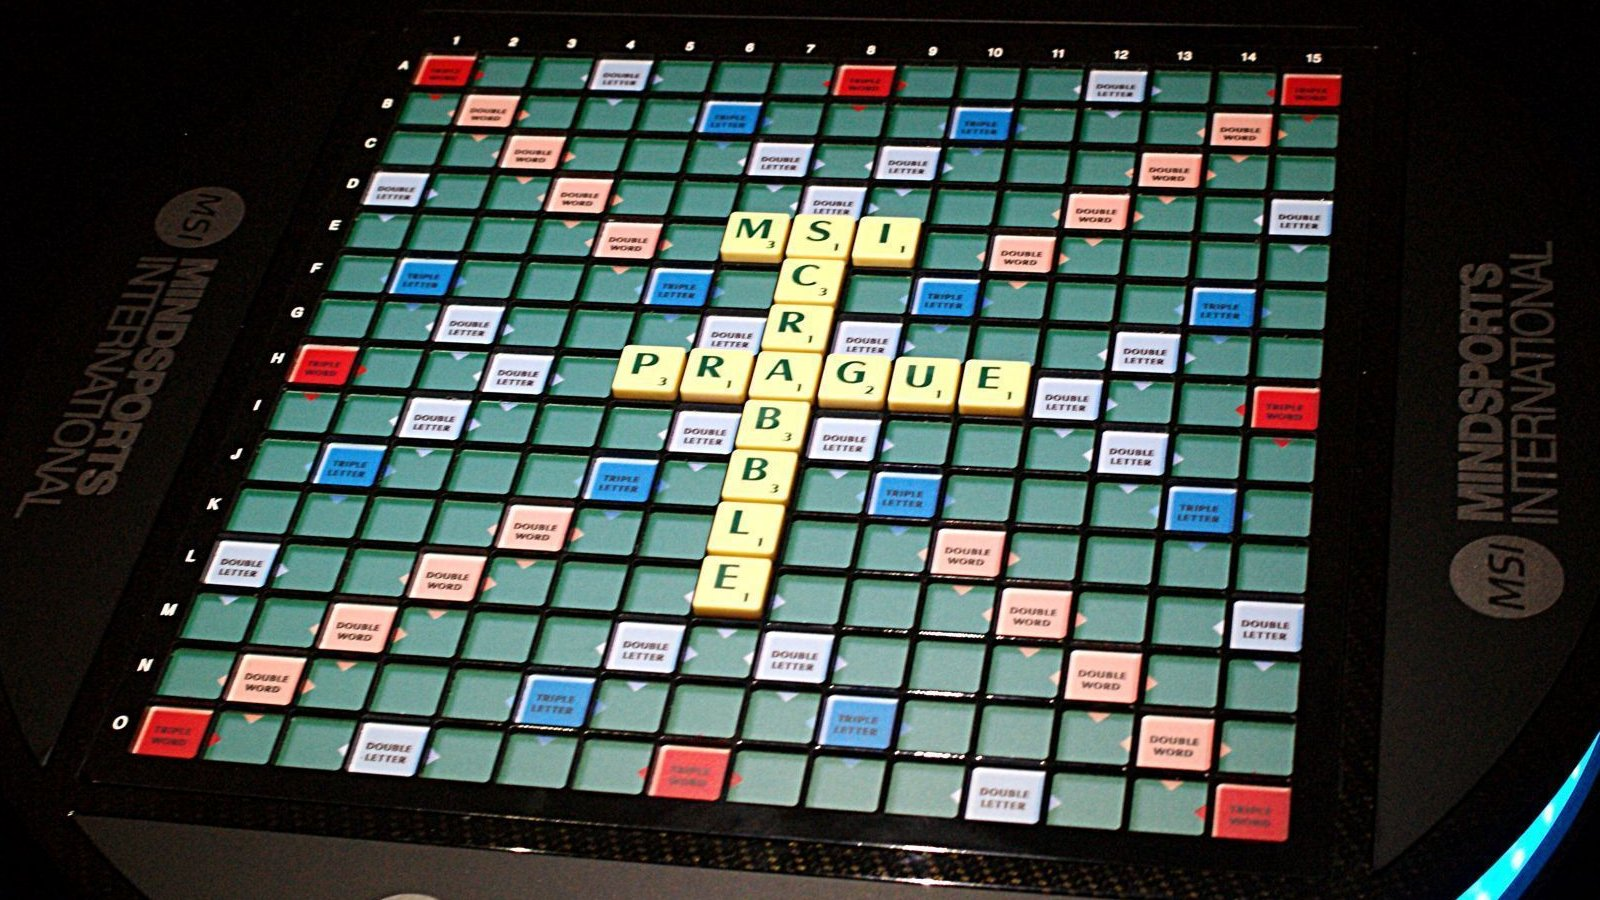
\includegraphics[scale=0.17]{graphics/board.jpg}
		\caption{Plansza wykonana z~włókna węglowego, podświetlana diodami LED.}
	\end{figure}
\end{frame}

\subsection{Ekstrakt z~SDM1}

\begin{frame}
	\frametitle{Przypomnienie (1/2)}

	Podczas poprzedniego wystąpienia zostały omówione następujące zagadnienia:

	\begin{enumerate}
		\item Porównanie słowników do gier dla języka polskiego:
			\begin{description}
				\item[OSPS] ,,Oficjalny Słownik Polskiego Scrabblisty''.
				\item[SA] Słownik alternatywny.
			\end{description}
		\item Analiza statystyczna słownika alternatywnego.
		\item Omówienie efektywnych struktur słownikowych zorientowanych na przeglądanie poprawnych sufiksów wyrazów:
			\begin{description}
				\item[Trie] Drzewo poszukiwań.
				\item[DAG] Directed Acyclic Graph.
				\item[GADDAG] prefiksowo-sufiksowa odmiana DAG.
			\end{description}
	\end{enumerate}
\end{frame}

\begin{frame}
	\frametitle{Przypomnienie (2/2)}

	Omówione zagadnienia - ciąg dalszy:

	\begin{enumerate}
		\setcounter{enumi}{3}
		\item Przedstawienie algorytmu Appela-Jacobsona wyznaczającego wszystkie legalne kombinacje ruchów dla ustalonego stanu gry.
		\item Podział rozgrywki na cztery fazy - MG, PEG-1, PEG-2, EG.
		\item Porównanie najlepszych algorytmów sztucznej inteligencji obecnej generacji:
			\begin{itemize}
				\item Algorytm Maven.
				\item Aplikacja Quackle.
			\end{itemize}
		\item Przedstawienie wybranych elementów algorytmu używanego w~aplikacji Quackle.
	\end{enumerate}
\end{frame}

\subsection{Założenia}

\begin{frame}[t]
	\frametitle{Założenia algorytmu}
	
	Cel pracy oraz przyjęte założenia:

	\begin{itemize}
		\item Zwiększenie procentowej liczby wygranych najlepszych algorytmów obecnej generacji:
			\begin{itemize}
				\item Skuteczność mierzona w~starciu z~przeciwnikami klasy mistrzowskiej.
			\end{itemize}
		\item Algorytmem bazowym (oraz referencyjnym) jest wykorzystywany przez aplikację Quackle.
		\item Średni czas wykonania ruchu nie może być większy niż w~algorytmach obecnej generacji.
		\item Złożoność pamięciowa algorytmu nie jest istotna.
		\item Słownik dopuszczalnych wyrazów jest znany z~góry:
			\begin{itemize}
				\item Dodanie obsługi nowego języka wymaga przeprowadzenia automatycznej analizy, która może być operacją czasochłonną.
			\end{itemize}
	\end{itemize}
\end{frame}

\section{Podstawy teoretyczne}
\subsection{Strategia optymalna}

\begin{frame}
	\frametitle{Strategia optymalna}

	\begin{block}{Twierdzenie}	
		Istnieje optymalna strategia gry w~Scrabble.
	\end{block}

	\begin{block}{Przestrzeń stanów}	
		Stan rozgrywki po~danej turze opisują parametry $P$ - rozmieszczenie klocków na planszy oraz $Z$ - zagranie. Przejście między stanami determinuje zmiana $(\Delta P, \Delta Z)$.
	\end{block}

	\begin{block}{Dowód}	
		Dla dowolnej rozgrywki tworzymy graf możliwych stanów wychodząc 
		od stanu końcowego. Do stanu końcowego można wejść tylko poprzez skończoną liczbę legalnych zagrań. Rozumując iteracyjnie dochodzimy do stanu początkowego, na każdym etapie analizując skończoną liczbę przejść między stanami. Wynika z~tego, że ilość stanów jest skończona. Można więc w~każdym kroku wybrać optymalną strategię, która maksymalizuje prawdopodobieństwo wygranej.
	\end{block}
\end{frame}

\begin{frame}
	\frametitle{Strategia optymalna - ilustracja dowodu}
	
	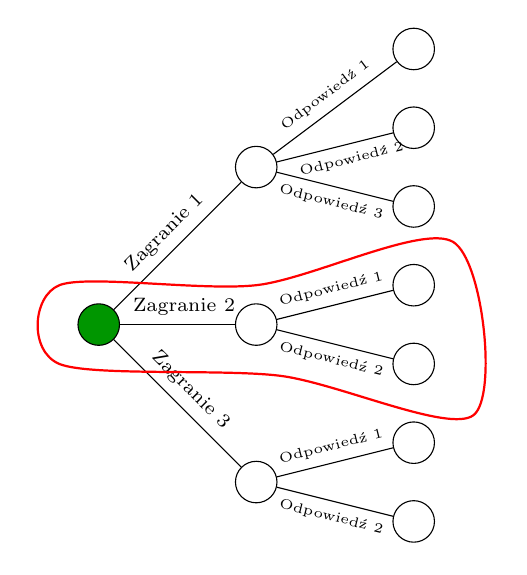
\begin{tikzpicture}
		\tikzstyle{state} = [draw, shape=circle, minimum width=15pt, minimum height=15pt]
		\node (s0) [state, fill=UniGreen] at (0,0) {};
		\node (s1) [state] at (2,2) {};
		\node (s2) [state] at (2,0) {};
		\node (s3) [state] at (2, -2) {};
		\node (s4) [state] at (4,3.5) {};
		\node (s5) [state] at (4,2.5) {};
		\node (s6) [state] at (4,1.5) {};
		\node (s7) [state] at (4,0.5) {};
		\node (s8) [state] at (4,-0.5) {};
		\node (s9) [state] at (4,-1.5) {};
		\node (s10) [state] at (4,-2.5) {};
		\draw (s0) -- node[above, sloped, font=\scriptsize] {Zagranie 1} (s1);
		\draw (s0) -- node[above, sloped, font=\scriptsize, near end, xshift=-8pt] {Zagranie 2} (s2);
		\draw (s0) -- node[above, sloped, font=\scriptsize] {Zagranie 3} (s3);
		\draw (s1) -- node[above, sloped, font=\tiny] {Odpowiedź 1} (s4);
		\draw (s1) -- node[xshift=-6pt, below, near end, sloped, font=\tiny] {Odpowiedź 2} (s5);
		\draw (s1) -- node[below, sloped, font=\tiny] {Odpowiedź 3} (s6);
		\draw (s2) -- node[above, sloped, font=\tiny] {Odpowiedź 1} (s7);
		\draw (s2) -- node[below, sloped, font=\tiny] {Odpowiedź 2} (s8);
		\draw (s3) -- node[above, sloped, font=\tiny] {Odpowiedź 1} (s9);
		\draw (s3) -- node[below, sloped, font=\tiny] {Odpowiedź 2} (s10);
		\draw [red, thick] plot [smooth cycle] coordinates {(-0.5, -0.5) (-0.5, 0.5) (2, 0.5) (4.5, 1.05) (4.76, -1.15) (2.3, -0.65)};
	\end{tikzpicture}
\end{frame}

\begin{frame}
	\frametitle{Strategia optymalna - następstwa}

	\begin{itemize}
		\item Wyznaczenie optymalnej strategii należy do klasy problemów \emph{PSPACE-complete}.
		\item Analiza przestrzeni stanów jest możliwa wyłącznie dla bardzo ograniczonej przestrzeni stanów:
			\begin{itemize}
				\item W~praktyce analiza przestrzeni stanów jest możliwa, gdy w~worku nie ma już klocków lub gdy pozostał jeden/dwa klocki.
			\end{itemize}
		\item \textbf{Należy zmieniać strategię w~zależności od fazy rozgrywki}:
			\begin{itemize}
				\item Nie zawsze można użyć strategii optymalnej.
				\item Wykorzystanie metod heurystycznych.
			\end{itemize}
	\end{itemize}
\end{frame}

\subsection{Fazy gry}

\begin{frame}
	\frametitle{Fazy gry}
	
	Rozgrywkę w~Scrabble można podzielić na cztery zasadnicze fazy:

	\begin{description}
		\item[OP] \emph{opening-play}. Faza obejmuje pierwsze zagranie.
		\item[MG] \emph{mid-game}. Faza trwa od momentu rozpoczęcia rozgrywki do momentu, w~którym w~worku pozostaje jeden/dwa klocki lub nie ma już klocków (w~zależności od przebiegu rozgrywki).
		\item[PEG] \emph{pre-endgame}. Faza trwa, gdy w~worku pozostał pojedynczy klocek. Według szacunków przez tę fazę przechodzi około $50\%$ gier. Można wyróżnić dwie podfazy:
			\begin{description}
				\item[PEG-1] W~worku pozostał jeden klocek.
				\item[PEG-2] W~worku pozostały dwa klocki.
			\end{description}
		\item[EG] \emph{end-game}. W~worku nie ma już żadnych klocków.
	\end{description}
\end{frame}

\captionsetup[figure]{skip=10pt}

\begin{frame}[fragile]
	\frametitle{Strategia a~faza gry}
	
	\begin{figure}
		\centering
		\begin{timeline}
			\Task[OP]{Maksymalizacja punktów uzyskanych z~zagrania otwierającego}
			\Task[MG]{Algorytm z~heurystyczną funkcją kosztu i~symulacją w~przód}
			\Task[EG]{Przeszukiwanie przestrzeni stanów (z~ograniczeniami)}
		\end{timeline}
		\caption{Zmiana strategii wraz z~progresją rozgrywki.}
	\end{figure}
\end{frame}

\section{Implementacja}
\subsection{Strategia}

\begin{frame}[fragile]
	\frametitle{Wzorzec projektowy - strategia}
	
	\begin{columns}
		\begin{column}{.5\textwidth}
			\begin{block}{Strategia}	
				Wzorzec definiuje rodzinę algorytmów, pakuje je jako osobne klasy i~powoduje, że są one w~pełni wymienne. Zastosowanie strategii pozwala na to, aby zmiany w~implementacji przetwarzania były całkowicie niezależne od strony klienta, który z~nich korzysta.
			\end{block}
		\end{column}
		\begin{column}{.5\textwidth}
			\scalebox{0.7}{
				\begin{tikzpicture}
					\umlclass[type=interface,x=0,y=3]{ScrabbleAI}{\# phase : GamePhase}{+ move() : void \\ \# pickStrategy() : IMoveStrategy} 
					\umlclass[type=interface,x=0,y=0]{IMoveStrategy}{}{+ move() : void} 
					\umlclass[x=-2, y=-2.25]{FirstPlayStrategy}{}{+ move() : void}
					\umlclass[x=0, y=-4.5]{MidGameStrategy}{}{+ move() : void}
					\umlclass[x=2, y=-2.25]{EndGameStrategy}{}{+ move() : void}
					\umluniassoc{ScrabbleAI}{IMoveStrategy}
					\umlimpl{IMoveStrategy}{FirstPlayStrategy}
					\umlimpl{IMoveStrategy}{MidGameStrategy}
					\umlimpl{IMoveStrategy}{EndGameStrategy}
				\end{tikzpicture}
			}
		\end{column}
	\end{columns}
\end{frame}

\subsection{Faza Opening Play}

\begin{frame}
	\frametitle{Otwarcie gry}

	\begin{itemize}
		\item Celem jest wybranie najwyżej punktowanego zagrania.
		\item W~algorytmie aplikacji Quackle jest przeszukiwany słownik i~dla każdej prawidłowej kombinacji liter wyznaczana jest wartość punktowa.
		\item Wprowadzona optymalizacja wydajnościowa:
			\begin{itemize}
				\item Ponieważ słownik jest znany z~góry można przeprowadzać wstępne obliczenia.
				\item Każdą możliwą kombinację liter indeksujemy 7-wyrazowym ciągiem znaków, które przedstawiają litery ułożone w~porządku alfabetycznym.
				\item Dla każdego indeksu obliczamy najlepsze otwarcie.
				\item Najlepsze otwarcie wyznaczane w~czasie jednostkowym (wyjątek: blanki).
			\end{itemize}
	\end{itemize}
\end{frame}

\subsection{Faza Mid Game}
\captionsetup[figure]{skip=2pt}

\begin{frame}
	\frametitle{Algorytm dla fazy mid-game}

	\begin{figure}
		\centering
			\scalebox{0.57}{
				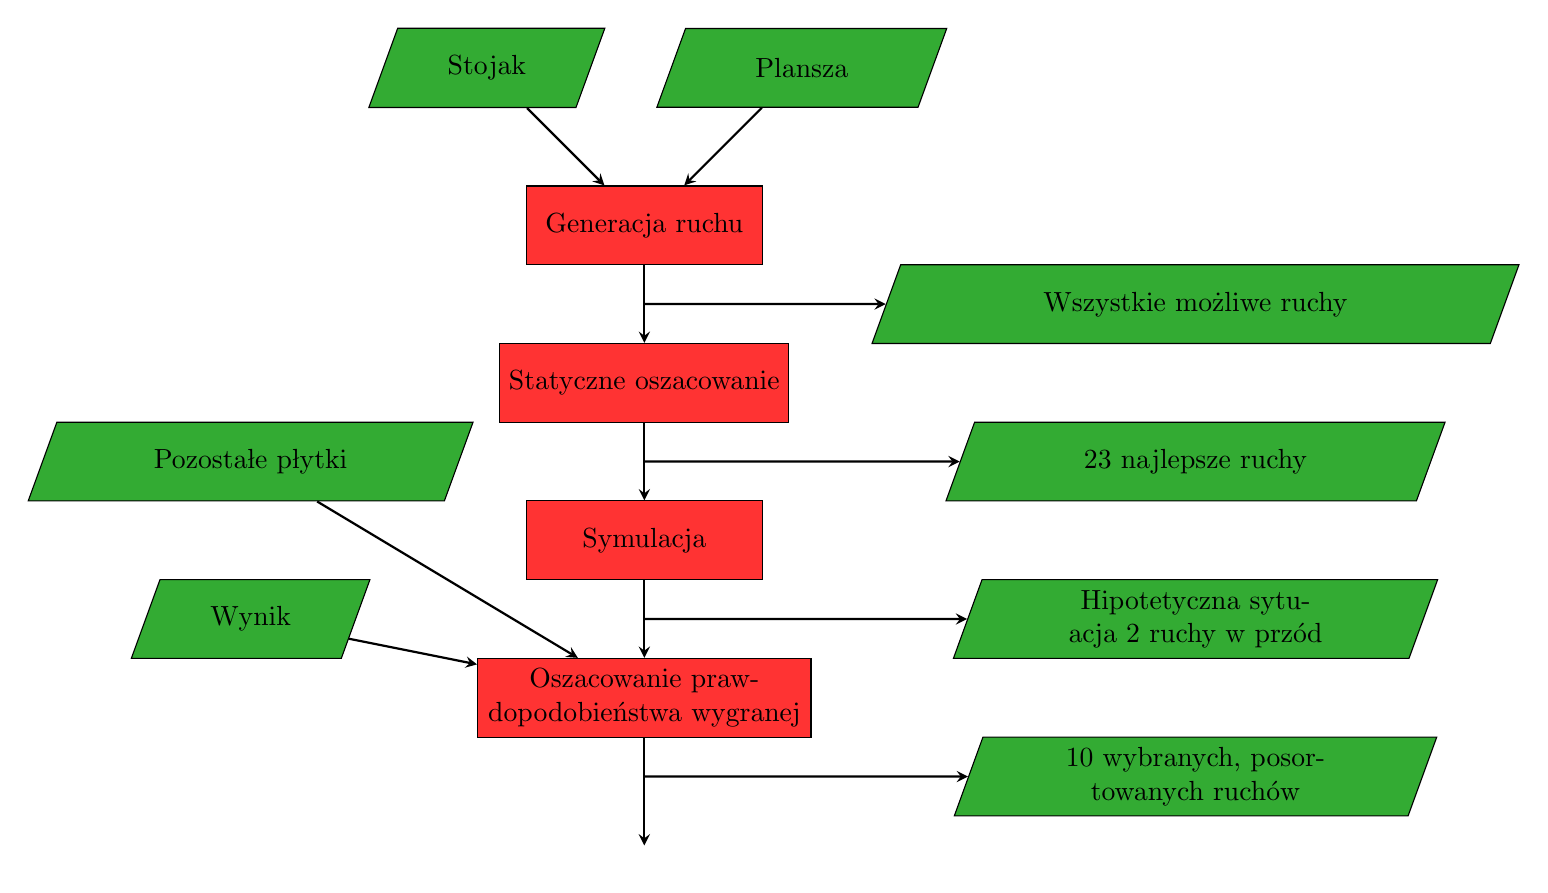
\begin{tikzpicture}[node distance=2cm]
					\noindent
					\tikzstyle{io} = [trapezium, trapezium left angle=70, trapezium right angle=110, minimum width=3cm, minimum height=1cm, text centered, draw=black, fill=UniGreen!80]
					\tikzstyle{process} = [rectangle, minimum width=3cm, minimum height=1cm, text centered, draw=black, fill=red!80]
					\tikzstyle{arrow} = [thick,->,>=stealth]
					
					\node (rack) [io] {Stojak};
					\node (board) [io, right of=rack, xshift=2cm] {Plansza};
					\coordinate (rackboard) at ($(rack)!0.5!(board)$);
					\node (movegen) [process, below of= rackboard] {Generacja ruchu};
					\node (staticeval) [process, below of=movegen] {Statyczne oszacowanie};
					\coordinate (movegenstaticeval) at ($(movegen)!0.5!(staticeval)$);
					\node (possmoves) [io, right of=movegenstaticeval, xshift=5cm] {Wszystkie możliwe ruchy};
					\node (simulation) [process, below of=staticeval] {Symulacja};
					\node (bestmoves) [io, below of=possmoves] {23 najlepsze ruchy};
					\node (hypsequences) [io, below of=bestmoves, text width=5cm] {Hipotetyczna sytuacja 2 ruchy w~przód};
					\node (winpercestimation) [process, below of=simulation, text width=4cm] {Oszacowanie prawdopodobieństwa wygranej};
					\node (end) [process, draw=none, fill=none, below of=winpercestimation, minimum height=1mm] { };
					\coordinate (staticevalsimulation) at ($(staticeval)!0.5!(simulation)$);
					\node (tilesleft) [io, left of=staticevalsimulation,xshift=-3cm] {Pozostałe płytki};
					\node (score) [io, below of=tilesleft] {Wynik};
					\coordinate (winpercestimationend) at ($(winpercestimation)!0.5!(end)$);
					\node (chosenmoves) [io, below of=hypsequences,text width=5cm] {10 wybranych, posortowanych ruchów};
					\draw [arrow] (movegen) -- (staticeval);
					\draw [arrow] (staticeval) -- (simulation);
					\draw [arrow] (simulation) -- (winpercestimation);
					\draw [arrow] (rack) -- (movegen);
					\draw [arrow] (board) -- (movegen);
					\draw [arrow] (winpercestimation) -- (end);
					\draw [arrow] (tilesleft) -- (winpercestimation);
					\draw [arrow] (score) -- (winpercestimation);
					\draw [arrow] ($(movegen)!0.5!(staticeval)$) -- (possmoves);
					\draw [arrow] ($(staticeval)!0.5!(simulation)$) -- (bestmoves);
					\draw [arrow] ($(simulation)!0.5!(winpercestimation)$) -- (hypsequences);
					\draw [arrow] ($(winpercestimation)!0.5!(end)$) -- (chosenmoves);
				\end{tikzpicture}
			}
			\caption{Schemat algorytmu referencyjnego dla fazy MG.}
	\end{figure}
\end{frame}

\begin{frame}
	\frametitle{Faza mid-game: Statyczne oszacowanie}
	
	Algorytm referencyjny wykorzystuje do statycznego oszacowania poniższą funkcję celu.

	\begin{block}{Funkcja celu}	
		$F(x) = P(x) + LV(x)$,
		\vskip5pt
		gdzie $P(x)$ to liczba punktów za zagranie $x$, a~$LV(x)$ to \emph{leave value} klocków pozostałych po wykonaniu zagrania $x$. 
	\end{block}

	\begin{block}{Leave value}	
		Obliczona na podstawie bazy danych gier wartość, która faworyzuje kombinacje liter o~większym prawdopodobieństwie dopełnienia wysokopunktowych zagrań w~nadchodzących ruchach. Może przyjmować dodatnie oraz ujemne wartości.
	\end{block}
\end{frame}

\begin{frame}
	\frametitle{Faza mid-game: Symulacja}

	Algorytm referencyjny wykonuje następującą symulację:

	\begin{enumerate}
		\item Gracz wykonuje zagranie $P_{1}$.
		\item Przeciwnik wybiera 7~losowych klocków, wyznacza wszystkie możliwości ruchu i~wykonuje zagranie $P_{2}$ dla ruchu z~najlepszym statycznym oszacowaniem.
		\item Gracz uzupełnia klocki, wyznacza wszystkie możliwości ruchu i~wykonuje zagranie $P_{3}$ dla ruchu z~najlepszym statycznym oszacowaniem.
		\item Gracz oblicza wartość $PV_{1}$ zagrania $P_{1}$ odejmując od liczby swoich punktów po zagraniu $P_{3}$ liczbę punktów przeciwnika po zagraniu $P_{2}$.
		\item Gracz dodaje do $PV_{1}$ \emph{leave value} po zagraniu $P_{3}$.
	\end{enumerate}
\end{frame}

\begin{frame}
	\frametitle{Faza mid-game: Oszacowanie prawdopodobieństwa wygranej}
	
	Algorytm referencyjny szacuje prawdopodobieństwo wygranej zgodnie z~poniższą zależnością.

	\begin{block}{Estymata prawdopodobieństwa wygranej}	
		$W: PV, TR \rightarrow [0;1]$,
		\vskip5pt
		gdzie $PV$ to wartość zagrania obliczona na etapie symulacji, a~$TR$ to liczba klocków pozostałych do wykorzystania w~partii.
	\end{block}

	Wartość funkcji jest wyznaczana na podstawie bazy danych gier.
\end{frame}

\begin{frame}
	\frametitle{Prawdopodobieństwo występowania bigramów}
	
	\begin{columns}
		\begin{column}{.5\textwidth}
			\begin{block}{N-gram}
				Sekwencja składająca się z n~liter, znaków lub wyrazów.
			\end{block}
			
		\begin{itemize}
			\item Unigram.
			\item Bigram.
			\item Trigram.
			\item 4-gram.
			\item ...
			\item N-gram.
		\end{itemize}
		
		\end{column}
		
		\begin{column}{.5\textwidth}
			\begin{tabular}{|c|c|}
				\hline
				Bigram	&	Wystąpienia	\\
				\hline
				ni		&	1 077 436	\\
				ie		&	1 028 249	\\
				ow	&	645 018		\\
				an		&	507 205		\\
				wa	&	484 295		\\
				za		&	313 370		\\
				po		&	301 636		\\
				ch		&	296 749		\\
				ał		&	294 734		\\
				ia		&	284 247		\\
				\hline
			\end{tabular}

		\end{column}

	\end{columns}

\end{frame}

\begin{frame}
	\frametitle{Prawdopodobieństwo występowania n-gramów}
	
	\begin{columns}
		\begin{column}{.3\textwidth}
			\scalebox{.8}{
				\begin{tabular}{|c|c|}
					\hline
					Trigram	&	Wystąpienia	\\
					\hline
					nie	&	635 196	\\
					owa	&	307 277	\\
					ani	&	195 186	\\
					wan	&	180 460	\\
					cie	&	148 513	\\
					nia	&	142 201	\\
					jąc	&	131 792	\\
					prz	&	130 283	\\
					wał	&	126 134	\\
					rze	&	116 370	\\
					\hline
				\end{tabular}
			}

		\end{column}
		
		\begin{column}{.3\textwidth}
			\scalebox{.8}{
				\begin{tabular}{|c|c|}
					\hline
					4-gram	&	Wystąpienia	\\
					\hline
					owan	&	127 626	\\
					ował		&	88 130		\\
					wani		&	78 095		\\
					niep		&	77 449		\\
					prze		&	73 230		\\
					ując		&	67 062		\\
					ania		&	61 398		\\
					ając		&	59 499		\\
					ście		&	56 462		\\
					łaby		&	55 380		\\
					\hline
				\end{tabular}
			}

		\end{column}
		
		\begin{column}{.3\textwidth}
			\scalebox{.8}{
				\begin{tabular}{|c|c|}
					\hline
					5-gram	&	Wystąpienia	\\
					\hline
					owani	&	54 991	\\
					niepo	&	40 329	\\
					ałaby	&	37 581	\\
					yście		&	33 161	\\
					owała	&	28 175	\\
					niewy	&	26 193	\\
					owane	&	25 555	\\
					wania	&	25 551	\\
					owany	&	25 542	\\
					ałyby	&	25 282	\\
					\hline
				\end{tabular}
			}

		\end{column}

	\end{columns}
\end{frame}

\begin{frame}
	\frametitle{Prawdopodobieństwo występowania n-gramów (2)}
	
	\begin{columns}
		\begin{column}{.5\textwidth}
				\begin{tabular}{|c|c|}
					\hline
					6-gram	&	Wystąpienia	\\
					\hline
					owania	&	17 609	\\
					wałaby	&	17 161	\\
					byście	&	16 821	\\
					liście		&	15 910	\\
					aniami	&	15 585	\\
					aniach	&	15 585	\\
					łyście	&	15 405	\\
					owanie	&	14 674	\\
					owałby	&	14 437	\\
					nieprz	&	14 328	\\
					\hline
				\end{tabular}
		\end{column}
		
		\begin{column}{.5\textwidth}
				\begin{tabular}{|c|c|}
					\hline
					7-gram	&	Wystąpienia	\\
					\hline
					owałaby	&	12 401		\\
					libyśmy		&	12 267		\\
					łybyśmy	&	12 094		\\
					ałyście		&	9 902		\\
					aliście		&	9 304		\\
					ibyście		&	8 445		\\
					libyści		&	8 443		\\
					ybyście		&	8 317		\\
					łybyści		&	8 314		\\
					nieprze		&	8 111		\\
					\hline
				\end{tabular}
		\end{column}
	\end{columns}
\end{frame}

\begin{frame}
	\frametitle{Najlepsze otwarcia}
	
	\begin{tikzpicture}
		\tikzstyle{every node}=[draw, shape=rectangle, rounded corners = 1pt, minimum width = 15pt, minimum height = 15pt, align=center, text height = 7pt];
		\node [fill=Board] at (0, 0) { };
		\node [fill=Board] at (.6, 0) { };
		\node [fill=DoubleLetterBonus] at (1.2, 0) {x2};
		\node [fill=Board] at (1.8, 0) { };
		\node [fill=Board] at (2.4, 0) { };
		\node [fill=Board] at (3, 0) { };
		\node [fill=DoubleWordBonus] at (3.6, 0) { };
		\node [fill=Board] at (4.2, 0) { };
		\node [fill=Board] at (4.8, 0) { };
		\node [fill=Board] at (5.4, 0) { };
		\node [fill=DoubleLetterBonus] at (6, 0) {x2};
		\node [fill=Board] at (6.6, 0) { };
		\node [fill=Board] at (7.2, 0) { };		
		\node [shape=star, star points=8, rounded corners = 0pt, fill=black, text height = 0pt] at (3.6, 0) {};
		\node [fill=Tile] at (0, -.6) {P};
		\node [fill=Tile] at (.6, -.6) {Ó};
		\node [fill=Tile] at (1.2, -.6) {Ź};
		\node [fill=Tile] at (1.8, -.6) {N};
		\node [fill=Tile] at (2.4, -.6) {O};
		\node [fill=Tile] at (3, -.6) {Ś};
		\node [fill=Tile] at (3.6, -.6) {Ć};
		\node [fill=Board] at (4.2, -.6) { };
		\node [fill=Board] at (4.8, -.6) { };
		\node [fill=Board] at (5.4, -.6) { };
		\node [fill=DoubleLetterBonus] at (6, -.6) {x2};
		\node [fill=Board] at (6.6, -.6) { };
		\node [fill=Board] at (7.2, -.6) { };	
		\node [draw=none, fill=none, align=left, text width=55pt] at (8.6, -.6) {126 punktów};
		\node [fill=Board] at (0, -1.2) { };
		\node [fill=Board] at (.6, -1.2) { };
		\node [fill=DoubleLetterBonus] at (1.2, -1.2) {x2};
		\node [fill=Board] at (1.8, -1.2) { };
		\node [fill=Board] at (2.4, -1.2) { };
		\node [fill=Board] at (3, -1.2) { };
		\node [fill=Tile] at (3.6, -1.2) {B};
		\node [fill=Tile] at (4.2, -1.2) {Ł};
		\node [fill=Tile] at (4.8, -1.2) {Ą};
		\node [fill=Tile] at (5.4, -1.2) {D};
		\node [fill=Tile] at (6, -1.2) {Ź};
		\node [fill=Tile] at (6.6, -1.2) {Ż};
		\node [fill=Tile] at (7.2, -1.2) {E};
		\node [draw=none, fill=none, align=left, text width=55pt] at (8.6, -1.2) {124 punkty};
		\node [fill=Board] at (0, -1.8) { };
		\node [fill=Board] at (.6, -1.8) { };
		\node [fill=DoubleLetterBonus] at (1.2, -1.8) {x2};
		\node [fill=Board] at (1.8, -1.8) { };
		\node [fill=Board] at (2.4, -1.8) { };
		\node [fill=Board] at (3, -1.8) { };
		\node [fill=Tile] at (3.6, -1.8) {U};
		\node [fill=Tile] at (4.2, -1.8) {B};
		\node [fill=Tile] at (4.8, -1.8) {O};
		\node [fill=Tile] at (5.4, -1.8) {D};
		\node [fill=Tile] at (6, -1.8) {Ź};
		\node [fill=Tile] at (6.6, -1.8) {Ż};
		\node [fill=Tile] at (7.2, -1.8) {E};		
		\node [draw=none, fill=none, align=left, text width=55pt] at (8.6, -1.8) {124 punkty};
		\node [fill=Board] at (0, -2.4) { };
		\node [fill=Board] at (.6, -2.4) { };
		\node [fill=DoubleLetterBonus] at (1.2, -2.4) {x2};
		\node [fill=Board] at (1.8, -2.4) { };
		\node [fill=Board] at (2.4, -2.4) { };
		\node [fill=Board] at (3, -2.4) { };
		\node [fill=Tile] at (3.6, -2.4) {P};
		\node [fill=Tile] at (4.2, -2.4) {Ó};
		\node [fill=Tile] at (4.8, -2.4) {J};
		\node [fill=Tile] at (5.4, -2.4) {D};
		\node [fill=Tile] at (6, -2.4) {Ź};
		\node [fill=Tile] at (6.6, -2.4) {K};
		\node [fill=Tile] at (7.2, -2.4) {Ę};		
		\node [draw=none, fill=none, align=left, text width=55pt] at (8.6, -2.4) {124 punkty};
		\node [fill=Board] at (0, -3) { };
		\node [fill=Board] at (.6, -3) { };
		\node [fill=DoubleLetterBonus] at (1.2, -3) {x2};
		\node [fill=Board] at (1.8, -3) { };
		\node [fill=Board] at (2.4, -3) { };
		\node [fill=Board] at (3, -3) { };
		\node [fill=Tile] at (3.6, -3) {G};
		\node [fill=Tile] at (4.2, -3) {Ł};
		\node [fill=Tile] at (4.8, -3) {Ó};
		\node [fill=Tile] at (5.4, -3) {D};
		\node [fill=Tile] at (6, -3) {Ź};
		\node [fill=Tile] at (6.6, -3) {Ż};
		\node [fill=Tile] at (7.2, -3) {E};		
		\node [draw=none, fill=none, align=left, text width=55pt] at (8.6, -3) {124 punkty};
		\node [fill=Board] at (0, -3.6) { };
		\node [fill=Board] at (.6, -3.6) { };
		\node [fill=DoubleLetterBonus] at (1.2, -3.6) {x2};
		\node [fill=Board] at (1.8, -3.6) { };
		\node [fill=Board] at (2.4, -3.6) { };
		\node [fill=Board] at (3, -3.6) { };
		\node [fill=Tile] at (3.6, -3.6) {U};
		\node [fill=Tile] at (4.2, -3.6) {B};
		\node [fill=Tile] at (4.8, -3.6) {Ą};
		\node [fill=Tile] at (5.4, -3.6) {D};
		\node [fill=Tile] at (6, -3.6) {Ź};
		\node [fill=Tile] at (6.6, -3.6) {Ż};
		\node [fill=Tile] at (7.2, -3.6) {E};		
		\node [draw=none, fill=none, align=left, text width=55pt] at (8.6, -3.6) {124 punkty};
		\node [fill=Board] at (0, -4.2) { };
		\node [fill=Board] at (.6, -4.2) { };
		\node [fill=DoubleLetterBonus] at (1.2, -4.2) {x2};
		\node [fill=Board] at (1.8, -4.2) { };
		\node [fill=Board] at (2.4, -4.2) { };
		\node [fill=Board] at (3, -4.2) { };
		\node [fill=Tile] at (3.6, -4.2) {U};
		\node [fill=Tile] at (4.2, -4.2) {G};
		\node [fill=Tile] at (4.8, -4.2) {Ó};
		\node [fill=Tile] at (5.4, -4.2) {D};
		\node [fill=Tile] at (6, -4.2) {Ź};
		\node [fill=Tile] at (6.6, -4.2) {Ż};
		\node [fill=Tile] at (7.2, -4.2) {E};		
		\node [draw=none, fill=none, align=left, text width=55pt] at (8.6, -4.2) {124 punkty};
		\node [fill=Board] at (0, -4.8) { };
		\node [fill=Board] at (.6, -4.8) { };
		\node [fill=DoubleLetterBonus] at (1.2, -4.8) {x2};
		\node [fill=Board] at (1.8, -4.8) { };
		\node [fill=Board] at (2.4, -4.8) { };
		\node [fill=Board] at (3, -4.8) { };
		\node [fill=Tile] at (3.6, -4.8) {B};
		\node [fill=Tile] at (4.2, -4.8) {L};
		\node [fill=Tile] at (4.8, -4.8) {U};
		\node [fill=Tile] at (5.4, -4.8) {Ź};
		\node [fill=Tile] at (6, -4.8) {Ń};
		\node [fill=Tile] at (6.6, -4.8) {Ż};
		\node [fill=Tile] at (7.2, -4.8) {E};		
		\node [draw=none, fill=none, align=left, text width=55pt] at (8.6, -4.8) {124 punkty};
		\node [fill=Board] at (0, -5.4) { };
		\node [fill=Board] at (.6, -5.4) { };
		\node [fill=DoubleLetterBonus] at (1.2, -5.4) {x2};
		\node [fill=Board] at (1.8, -5.4) { };
		\node [fill=Board] at (2.4, -5.4) { };
		\node [fill=Board] at (3, -5.4) { };
		\node [fill=Tile] at (3.6, -5.4) {P};
		\node [fill=Tile] at (4.2, -5.4) {Ó};
		\node [fill=Tile] at (4.8, -5.4) {J};
		\node [fill=Tile] at (5.4, -5.4) {D};
		\node [fill=Tile] at (6, -5.4) {Ź};
		\node [fill=Tile] at (6.6, -5.4) {K};
		\node [fill=Tile] at (7.2, -5.4) {Ą};		
		\node [draw=none, fill=none, align=left, text width=55pt] at (8.6, -5.4) {124 punkty};
		\node [fill=Board] at (0, -6) { };
		\node [fill=Board] at (.6, -6) { };
		\node [fill=DoubleLetterBonus] at (1.2, -6) {x2};
		\node [fill=Board] at (1.8, -6) { };
		\node [fill=Board] at (2.4, -6) { };
		\node [fill=Tile] at (3, -6) {U};
		\node [fill=Tile] at (3.6, -6) {G};
		\node [fill=Tile] at (4.2, -6) {R};
		\node [fill=Tile] at (4.8, -6) {Z};
		\node [fill=Tile] at (5.4, -6) {Ą};
		\node [fill=Tile] at (6, -6) {Ź};
		\node [fill=Tile] at (6.6, -6) {Ć};
		\node [fill=Board] at (7.2, -6) { };		
		\node [draw=none, fill=none, align=left, text width=55pt] at (8.6, -6) {124 punkty};
	\end{tikzpicture}
\end{frame}

\begin{frame}
	\frametitle{Najlepsze kombinacje liter}
	
		Najlepsze kombinacje liter to zawartość stojaka, która umożliwia ułożenie (niezależnie) jak największej ilości słów.
	
		\vspace{1em}
	
		\begin{columns}
		\begin{column}{.5\textwidth}
			\scalebox{.8}{
				\begin{tabular}{|c|c|}
					\hline
					6 liter	&	Kombinacje	\\
					\hline
					e, m, n, o, r, t	&	10 wyrazów	\\
					a, i, k, l, n, o		&	10 wyrazów	\\
					a, e, i, l, m, n	&	10 wyrazów	\\
					e, i, k, m, o, s	&	9 wyrazów	\\
					a, i, k, m, n, o	&	9 wyrazów	\\
					a, i, l, m, o, s	&	9 wyrazów	\\
					a, i, k, o, t, w	&	9 wyrazów	\\
					a, i, k, n, t, u		&	9 wyrazów	\\
					a, e, k, l, s, z		&	9 wyrazów	\\
					a, e, i, k, m, r	&	9 wyrazów	\\
					\hline
				\end{tabular}
			}

		\end{column}
		
		\begin{column}{.5\textwidth}
			\scalebox{.8}{
				\begin{tabular}{|c|c|}
					\hline
					7 liter	&	Kombinacje	\\
					\hline
					e, i, k, l, n, o, w	&	12 wyrazów	\\
					a, e, i, k, p, r, s	&	12 wyrazów	\\
					a, e, i, k, l, n, p	&	12 wyrazów	\\
					a, e, k, n, r, t, y	&	11 wyrazów	\\
					a, i, k, m, o, p, s&	11 wyrazów	\\
					a, i, k, m, o, r, w&	11 wyrazów	\\
					a, a, i, k, l, m, s	&	10 wyrazów	\\
					a, i, k, m, o, s, t&	10 wyrazów	\\
					a, i, k, l, n, o, w	&	10 wyrazów	\\
					a, i, k, l, m, n, o&	10 wyrazów	\\
					\hline
				\end{tabular}
			}

		\end{column}
	\end{columns}
\end{frame}

\section{Algorytmy i~struktury danych}
\subsection{Wyznaczanie możliwych ruchów}

\begin{frame}
	\frametitle{Wyznaczanie wszystkich legalnych ruchów}
	
	\begin{columns}
		\begin{column}{.5\textwidth}
		
			\begin{itemize}
				\item Algorytm opisany w~pracy \emph{The World's Fastest Scrabble Program} A.~W.~Appela i~G.~J.~Jacobsona.
				\item Algorytm z~nawrotami.
				\item Bazuje na skompresowanej, grafowej odmianie drzewa \emph{trie} o~nazwie \textbf{DAWG} (ang. \textbf{D}irected \textbf{A}cyclic \textbf{W}ord \textbf{G}raph).
			\end{itemize}
			
		\end{column}
		
		\begin{column}{.5\textwidth}
			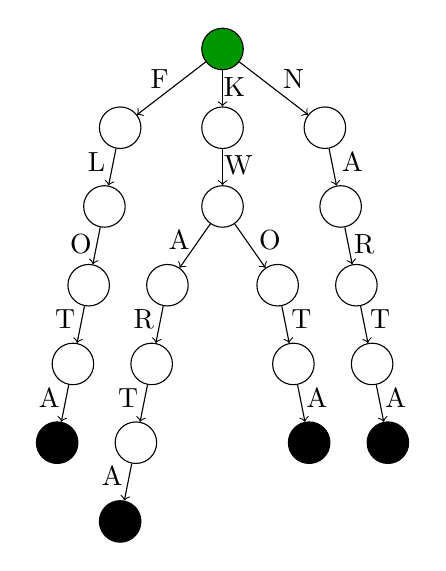
\begin{tikzpicture}
				\tikzstyle{every node}=[draw, shape=circle, minimum width = 15pt, minimum height = 15pt, text height = 0pt];
				\node [fill=UniGreen] (root) at (0,0) {};
				\node (n01) at (-1.3,-1) {};
				\node (n02) at (0, -1) {};
				\node (n03) at (1.3, -1) {};
				\node [draw=none] (t01) at (-0.8, -0.5) {F};
				\node [draw=none] (t02) at (0.15, -0.6) {K};
				\node [draw=none] (t01) at (0.9, -0.5) {N};
				\draw[->] (root) -- (n01);
				\draw[->] (root) -- (n02);
				\draw[->] (root) -- (n03);
				\node (n11) at (-1.5, -2) {};
				\node (n12) at (0, -2) {};
				\node (n13) at (1.5, -2) {};
				\node [draw=none] (t11) at (-1.6, -1.55) {L};
				\node [draw=none] (t12) at (0.2, -1.6) {W};
				\node [draw=none] (t13) at (1.65, -1.55) {A};
				\draw[->] (n01) -- (n11);
				\draw[->] (n02) -- (n12);
				\draw[->] (n03) -- (n13);
				\node (n21) at (-1.7, -3) {};
				\node (n22) at (-0.7, -3) {};
				\node (n23) at (0.7, -3) {};
				\node (n24) at (1.7, -3) {};
				\node [draw=none] (t21) at (-1.8, -2.6) {O};
				\node [draw=none] (t22) at (-0.55, -2.55) {A};
				\node [draw=none] (t23) at (0.6, -2.55) {O};
				\node [draw=none] (t23) at (1.8, -2.6) {R};
				\draw[->] (n11) -- (n21);
				\draw[->] (n12) -- (n22);
				\draw[->] (n12) -- (n23);
				\draw[->] (n13) -- (n24);
				\node (n31) at (-1.9, -4) {};
				\node (n32) at (-0.9, -4) {};
				\node (n33) at (0.9, -4) {};
				\node (n34) at (1.9, -4) {};
				\node [draw=none] (t31) at (-2.0, -3.55) {T};
				\node [draw=none] (t32) at (-1.0, -3.55) {R};
				\node [draw=none] (t33) at (1.0, -3.55) {T};
				\node [draw=none] (t33) at (2.0, -3.55) {T};
				\draw[->] (n21) -- (n31);
				\draw[->] (n22) -- (n32);
				\draw[->] (n23) -- (n33);
				\draw[->] (n24) -- (n34);
				\node [draw=none] (t41) at (-2.2, -4.55) {A};
				\node [draw=none] (t42) at (-1.2, -4.55) {T};
				\node [draw=none] (t43) at (1.2, -4.55) {A};
				\node [draw=none] (t43) at (2.2, -4.55) {A};
				\node [fill=black] (n41) at (-2.1, -5) {};
				\node (n42) at (-1.1, -5) {};
				\node [fill=black] (n43) at (1.1, -5) {};
				\node [fill=black] (n44) at (2.1, -5) {};
				\draw[->] (n31) -- (n41);
				\draw[->] (n32) -- (n42);
				\draw[->] (n33) -- (n43);
				\draw[->] (n34) -- (n44);
				\node [fill=black] (n52) at (-1.3, -6) {};
				\node [draw=none] (t32) at (-1.4, -5.55) {A};
				\draw[->] (n42) -- (n52);
			\end{tikzpicture}
		\end{column}
	\end{columns}
\end{frame}

\begin{frame}
	\frametitle{Trie vs DAWG}
	
	\begin{columns}
	\begin{column}{.55\textwidth}
			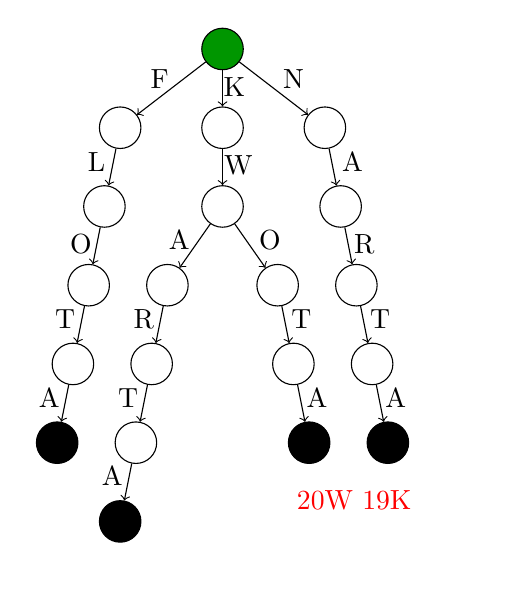
\begin{tikzpicture}
				\tikzstyle{every node}=[draw, shape=circle, minimum width = 15pt, minimum height = 15pt, text height = 0pt];
				\node [fill=UniGreen] (root) at (0,0) {};
				\node (n01) at (-1.3,-1) {};
				\node (n02) at (0, -1) {};
				\node (n03) at (1.3, -1) {};
				\node [draw=none] (t01) at (-0.8, -0.5) {F};
				\node [draw=none] (t02) at (0.15, -0.6) {K};
				\node [draw=none] (t01) at (0.9, -0.5) {N};
				\draw[->] (root) -- (n01);
				\draw[->] (root) -- (n02);
				\draw[->] (root) -- (n03);
				\node (n11) at (-1.5, -2) {};
				\node (n12) at (0, -2) {};
				\node (n13) at (1.5, -2) {};
				\node [draw=none] (t11) at (-1.6, -1.55) {L};
				\node [draw=none] (t12) at (0.2, -1.6) {W};
				\node [draw=none] (t13) at (1.65, -1.55) {A};
				\draw[->] (n01) -- (n11);
				\draw[->] (n02) -- (n12);
				\draw[->] (n03) -- (n13);
				\node (n21) at (-1.7, -3) {};
				\node (n22) at (-0.7, -3) {};
				\node (n23) at (0.7, -3) {};
				\node (n24) at (1.7, -3) {};
				\node [draw=none] (t21) at (-1.8, -2.6) {O};
				\node [draw=none] (t22) at (-0.55, -2.55) {A};
				\node [draw=none] (t23) at (0.6, -2.55) {O};
				\node [draw=none] (t23) at (1.8, -2.6) {R};
				\draw[->] (n11) -- (n21);
				\draw[->] (n12) -- (n22);
				\draw[->] (n12) -- (n23);
				\draw[->] (n13) -- (n24);
				\node (n31) at (-1.9, -4) {};
				\node (n32) at (-0.9, -4) {};
				\node (n33) at (0.9, -4) {};
				\node (n34) at (1.9, -4) {};
				\node [draw=none] (t31) at (-2.0, -3.55) {T};
				\node [draw=none] (t32) at (-1.0, -3.55) {R};
				\node [draw=none] (t33) at (1.0, -3.55) {T};
				\node [draw=none] (t33) at (2.0, -3.55) {T};
				\draw[->] (n21) -- (n31);
				\draw[->] (n22) -- (n32);
				\draw[->] (n23) -- (n33);
				\draw[->] (n24) -- (n34);
				\node [draw=none] (t41) at (-2.2, -4.55) {A};
				\node [draw=none] (t42) at (-1.2, -4.55) {T};
				\node [draw=none] (t43) at (1.2, -4.55) {A};
				\node [draw=none] (t43) at (2.2, -4.55) {A};
				\node [fill=black] (n41) at (-2.1, -5) {};
				\node (n42) at (-1.1, -5) {};
				\node [fill=black] (n43) at (1.1, -5) {};
				\node [fill=black] (n44) at (2.1, -5) {};
				\draw[->] (n31) -- (n41);
				\draw[->] (n32) -- (n42);
				\draw[->] (n33) -- (n43);
				\draw[->] (n34) -- (n44);
				\node [fill=black] (n52) at (-1.3, -6) {};
				\node [draw=none] (t32) at (-1.4, -5.55) {A};
				\draw[->] (n42) -- (n52);
				\node [draw=none, color=red, text width=60pt, text height=20pt] (label) at (2, -5.5) {20W 19K};
			\end{tikzpicture}
		\end{column}
		\begin{column}{.5\textwidth}
			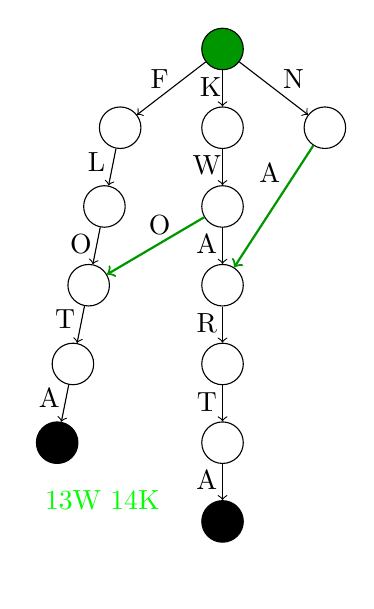
\begin{tikzpicture}
				\tikzstyle{every node}=[draw, shape=circle, minimum width = 15pt, minimum height = 15pt, text height = 0pt];
				\node [fill=UniGreen] (root) at (0,0) {};
				\node (n01) at (-1.3,-1) {};
				\node (n02) at (0, -1) {};
				\node (n03) at (1.3, -1) {};
				\node [draw=none] (t01) at (-0.8, -0.5) {F};
				\node [draw=none] (t02) at (-0.15, -0.6) {K};
				\node [draw=none] (t01) at (0.9, -0.5) {N};
				\draw[->] (root) -- (n01);
				\draw[->] (root) -- (n02);
				\draw[->] (root) -- (n03);
				\node (n11) at (-1.5, -2) {};
				\node (n12) at (0, -2) {};
				\node [draw=none] (t11) at (-1.6, -1.55) {L};
				\node [draw=none] (t12) at (-0.2, -1.6) {W};
				\node [draw=none] (t23) at (0.6, -1.7) {A};
				\draw[->] (n01) -- (n11);
				\draw[->] (n02) -- (n12);
				\node (n21) at (-1.7, -3) {};
				\node (n22) at (0, -3) {};
				\node [draw=none] (t21) at (-1.8, -2.6) {O};
				\node [draw=none] (t22) at (-0.8, -2.35) {O};
				\node [draw=none] (t23) at (-0.2, -2.6) {A};
				\draw[->] (n11) -- (n21);
				\draw[->, color=UniGreen, thick] (n12) -- (n21);
				\draw[->] (n12) -- (n22);
				\draw[->, color=UniGreen, thick] (n03) -- (n22);
				\node (n31) at (-1.9, -4) {};
				\node (n32) at (0, -4) {};
				\node [draw=none] (t31) at (-2.0, -3.55) {T};
				\node [draw=none] (t32) at (-0.2, -3.6) {R};
				\draw[->] (n21) -- (n31);
				\draw[->] (n22) -- (n32);
				\node [fill=black] (n41) at (-2.1, -5) {};
				\node (n42) at (0, -5) {};
				\node [draw=none] (t41) at (-2.2, -4.55) {A};
				\node [draw=none] (t42) at (-0.2, -4.6) {T};
				\draw[->] (n31) -- (n41);
				\draw[->] (n32) -- (n42);
				\node [fill=black] (n51) at (0, -6) {};
				\node [draw=none] (t51) at (-0.2, -5.6) {A};
				\draw[->] (n42) -- (n51);
				\node [draw=none, color=green, text width=60pt, text height=20pt] (label) at (-1.2, -5.5) {13W 14K};
			\end{tikzpicture}
		\end{column}
	\end{columns}
\end{frame}

\begin{frame}
	\frametitle{Algorytm Appela-Jacobsona (1)}
	
	\begin{enumerate}
		\item Redukcja złożoności problemu do jednego wymiaru:
			\begin{itemize}
				\item rozpatrywanie ruchów wyłącznie poziomo,
				\item ograniczenie zbioru wyłącznie do jednego wiersza.
			\end{itemize}
		
		Rozumowanie należy powtórzyć dla wszystkich wierszy, a~następnie transponować planszę i~zastosować do ruchów w~pionie.
	\end{enumerate}
	
	\begin{center}
		\scalebox{0.9}{
			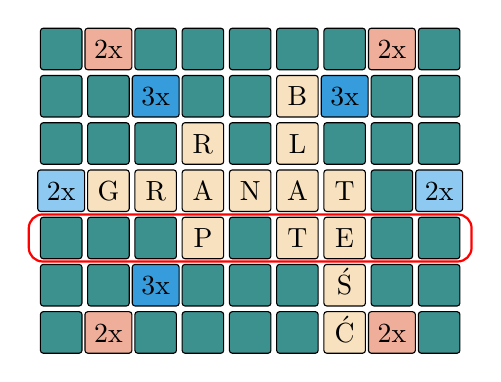
\begin{tikzpicture}
			\tikzstyle{every node}=[draw, shape=rectangle, rounded corners = 1pt, minimum width = 15pt, minimum height = 15pt, align=center, text height = 7pt];
			\node [fill=Board] at (-0.6, 0) {};
			\node [fill=DoubleWordBonus] at (0, 0) {2x};
			\node [fill=Board] at (0.6, 0) {};
			\node [fill=Board] at (1.2, 0) {};
			\node [fill=Board] at (1.8, 0) {};
			\node [fill=Board] at (2.4, 0) {};
			\node [fill=Board] at (3.0, 0) {};
			\node [fill=DoubleWordBonus] at (3.6, 0) {2x};
			\node [fill=Board] at (4.2, 0) {};
			\node [fill=Board] at (-.6, -.6) {};
			\node [fill=Board] at (0, -.6) {};
			\node [fill=TripleLetterBonus] at (0.6, -.6) {3x};
			\node [fill=Board] at (1.2, -.6) {};
			\node [fill=Board] at (1.8, -.6) {};
			\node [fill=Tile] at (2.4, -.6) {B};
			\node [fill=TripleLetterBonus] at (3.0, -.6) {3x};
			\node [fill=Board] at (3.6, -.6) {};
			\node [fill=Board] at (4.2, -.6) {};
			\node [fill=Board] at (-.6, -1.2) {};
			\node [fill=Board] at (0, -1.2) {};
			\node [fill=Board] at (0.6, -1.2) {};
			\node [fill=Tile] at (1.2, -1.2) {R};
			\node [fill=Board] at (1.8, -1.2) {};
			\node [fill=Tile] at (2.4, -1.2) {L};
			\node [fill=Board] at (3.0, -1.2) {};
			\node [fill=Board] at (3.6, -1.2) {};
			\node [fill=Board] at (4.2, -1.2) {};
			\node [fill=DoubleLetterBonus] at (-.6, -1.8) {2x};
			\node [fill=Tile] at (0, -1.8) {G};
			\node [fill=Tile] at (.6, -1.8) {R};
			\node [fill=Tile] at (1.2, -1.8) {A};
			\node [fill=Tile] at (1.8, -1.8) {N};
			\node [fill=Tile] at (2.4, -1.8) {A};
			\node [fill=Tile] at (3.0, -1.8) {T};
			\node [fill=Board] at (3.6, -1.8) {};
			\node [fill=DoubleLetterBonus] at (4.2, -1.8) {2x};
			\node [fill=Board] at (-.6, -2.4) {};
			\node [fill=Board] at (0, -2.4) {};
			\node [fill=Board] at (0.6, -2.4) {};
			\node [fill=Tile] at (1.2, -2.4) {P};
			\node [fill=Board] at (1.8, -2.4) {};
			\node [fill=Tile] at (2.4, -2.4) {T};
			\node [fill=Tile] at (3.0, -2.4) {E};
			\node [fill=Board] at (3.6, -2.4) {};
			\node [fill=Board] at (4.2, -2.4) {};
			\node [fill=Board] at (-.6, -3.0) {};
			\node [fill=Board] at (0, -3.0) {};
			\node [fill=TripleLetterBonus] at (0.6, -3.0) {3x};
			\node [fill=Board] at (1.2, -3.0) {};
			\node [fill=Board] at (1.8, -3.0) {};
			\node [fill=Board] at (2.4, -3.0) {};
			\node [fill=Tile] at (3.0, -3.0) {Ś};
			\node [fill=Board] at (3.6, -3.0) {};
			\node [fill=Board] at (4.2, -3.0) {};
			\node [fill=Board] at (-.6, -3.6) {};
			\node [fill=DoubleWordBonus] at (0, -3.6) {2x};
			\node [fill=Board] at (0.6, -3.6) {};
			\node [fill=Board] at (1.2, -3.6) {};
			\node [fill=Board] at (1.8, -3.6) {};
			\node [fill=Board] at (2.4, -3.6) {};
			\node [fill=Tile] at (3.0, -3.6) {Ć};
			\node [fill=DoubleWordBonus] at (3.6, -3.6) {2x};
			\node [fill=Board] at (4.2, -3.6) {};
			\node [draw, thick, shape = rectangle, rounded corners = 5pt, color = red, fill = none, minimum height = 17 pt, minimum width = 160 pt] at (1.8, -2.4) {};
		\end{tikzpicture}
	}
	\end{center}
\end{frame}

\begin{frame}
	\frametitle{Algorytm Appela-Jacobsona (2)}
	
	\begin{enumerate}
		\setcounter{enumi}{1}
		\item Ograniczenie zbioru znaków możliwych do wstawienia w~miejsce pustych płytek:
			\begin{itemize}
				\item ruch w~danym kierunku może skutkować tworzeniem nowych słów w~kierunku przeciwnym,
				\item słowa utworzone w~kierunku przeciwnym powstają zawsze poprzez dodanie jednego znaku.
			\end{itemize}
	\end{enumerate}

	\begin{center}
		\scalebox{0.9}{
			\begin{tikzpicture}
			\tikzstyle{every node}=[draw, shape=rectangle, rounded corners = 1pt, minimum width = 15pt, minimum height = 15pt, align=center, text height = 7pt];
			\node [fill=Board] at (-0.6, 0) {};
			\node [fill=DoubleWordBonus] at (0, 0) {2x};
			\node [fill=Board] at (0.6, 0) {};
			\node [fill=Board] at (1.2, 0) {};
			\node [fill=Board] at (1.8, 0) {};
			\node [fill=Board] at (2.4, 0) {};
			\node [fill=Board] at (3.0, 0) {};
			\node [fill=DoubleWordBonus] at (3.6, 0) {2x};
			\node [fill=Board] at (4.2, 0) {};
			\node [fill=Board] at (-.6, -.6) {};
			\node [fill=Board] at (0, -.6) {};
			\node [fill=TripleLetterBonus] at (0.6, -.6) {3x};
			\node [fill=Board] at (1.2, -.6) {};
			\node [fill=Board] at (1.8, -.6) {};
			\node [fill=Tile] at (2.4, -.6) {B};
			\node [fill=TripleLetterBonus] at (3.0, -.6) {3x};
			\node [fill=Board] at (3.6, -.6) {};
			\node [fill=Board] at (4.2, -.6) {};
			\node [fill=Board] at (-.6, -1.2) {};
			\node [fill=Board] at (0, -1.2) {};
			\node [fill=Board] at (0.6, -1.2) {};
			\node [fill=Tile] at (1.2, -1.2) {R};
			\node [fill=Board] at (1.8, -1.2) {};
			\node [fill=Tile] at (2.4, -1.2) {L};
			\node [fill=Board] at (3.0, -1.2) {};
			\node [fill=Board] at (3.6, -1.2) {};
			\node [fill=Board] at (4.2, -1.2) {};
			\node [fill=DoubleLetterBonus] at (-.6, -1.8) {2x};
			\node [fill=Tile] at (0, -1.8) {G};
			\node [fill=Tile] at (.6, -1.8) {R};
			\node [fill=Tile] at (1.2, -1.8) {A};
			\node [fill=Tile] at (1.8, -1.8) {N};
			\node [fill=Tile] at (2.4, -1.8) {A};
			\node [fill=Tile] at (3.0, -1.8) {T};
			\node [fill=Board] at (3.6, -1.8) {};
			\node [fill=DoubleLetterBonus] at (4.2, -1.8) {2x};
			\node [fill=Board] at (-.6, -2.4) {};
			\node [fill=Board] (below_g_node) at (0, -2.4) {};
			\node [fill=Board] (below_r_node) at (0.6, -2.4) {};
			\node [fill=Tile] at (1.2, -2.4) {P};
			\node [fill=Board] at (1.8, -2.4) {};
			\node [fill=Tile] at (2.4, -2.4) {T};
			\node [fill=Tile] at (3.0, -2.4) {E};
			\node [fill=Board] at (3.6, -2.4) {};
			\node [fill=Board] at (4.2, -2.4) {};
			\node [fill=Board] at (-.6, -3.0) {};
			\node [fill=Board] at (0, -3.0) {};
			\node [fill=TripleLetterBonus] at (0.6, -3.0) {3x};
			\node [fill=Board] at (1.2, -3.0) {};
			\node [fill=Board] at (1.8, -3.0) {};
			\node [fill=Board] at (2.4, -3.0) {};
			\node [fill=Tile] at (3.0, -3.0) {Ś};
			\node [fill=Board] at (3.6, -3.0) {};
			\node [fill=Board] at (4.2, -3.0) {};
			\node [fill=Board] at (-.6, -3.6) {};
			\node [fill=DoubleWordBonus] at (0, -3.6) {2x};
			\node [fill=Board] at (0.6, -3.6) {};
			\node [fill=Board] at (1.2, -3.6) {};
			\node [fill=Board] at (1.8, -3.6) {};
			\node [fill=Board] at (2.4, -3.6) {};
			\node [fill=Tile] at (3.0, -3.6) {Ć};
			\node [fill=DoubleWordBonus] at (3.6, -3.6) {2x};
			\node [fill=Board] at (4.2, -3.6) {};
			\node [draw=none, minimum width=0pt, minimum height=0pt] (below_g_node_cover) at (0, -2.4) {};
			\node [draw=none, minimum width=0pt, minimum height=0pt] (below_r_node_cover) at (0.6, -2.4) {};
			\node [draw=none, minimum width=0pt, minimum height=0pt] (below_n_node_cover) at (1.8, -2.4) {};
			\node [draw, rectangle, color=UniGreen] (below_g_possibilities) at (-2.7, -1.7) {Ę, O, U};
			\node [draw, rectangle, color=UniGreen] (below_r_possibilities) at (-2, -3.5) {E, O};
			\node [draw, rectangle, color=UniGreen] (below_n_possibilities) at (6, -.4) {A, I, O, U, Y};
			\draw[->, color=UniGreen] (below_g_possibilities) -- (below_g_node_cover);
			\draw[->, color=UniGreen] (below_r_possibilities) -- (below_r_node_cover);
			\draw[->, color=UniGreen] (below_n_possibilities) -- (below_n_node_cover);
		\end{tikzpicture}
	}
	\end{center}
\end{frame}

\begin{frame}
	\frametitle{Algorytm Appela-Jacobsona (3)}
	
	\begin{enumerate}
		\setcounter{enumi}{2}
		\item Wyznaczenie kotwic (ang. \emph{anchors}):
			\begin{itemize}
				\item kotwica to najbardziej wysunięta na lewo płytka nowego słowa, która jest przyległa do płytki istniejącego już na planszy słowa,
				\item kotwicą może być każde puste miejsce przyległe do płytki znajdującej się na planszy.
			\end{itemize}
	\end{enumerate}

	\begin{center}
		\scalebox{0.9}{
			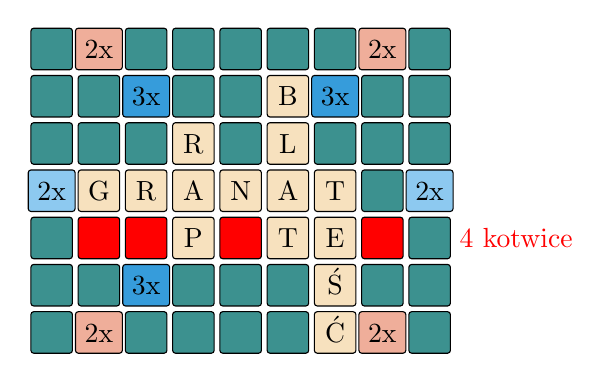
\begin{tikzpicture}
			\tikzstyle{every node}=[draw, shape=rectangle, rounded corners = 1pt, minimum width = 15pt, minimum height = 15pt, align=center, text height = 7pt];
			\node [fill=Board] at (-0.6, 0) {};
			\node [fill=DoubleWordBonus] at (0, 0) {2x};
			\node [fill=Board] at (0.6, 0) {};
			\node [fill=Board] at (1.2, 0) {};
			\node [fill=Board] at (1.8, 0) {};
			\node [fill=Board] at (2.4, 0) {};
			\node [fill=Board] at (3.0, 0) {};
			\node [fill=DoubleWordBonus] at (3.6, 0) {2x};
			\node [fill=Board] at (4.2, 0) {};
			\node [fill=Board] at (-.6, -.6) {};
			\node [fill=Board] at (0, -.6) {};
			\node [fill=TripleLetterBonus] at (0.6, -.6) {3x};
			\node [fill=Board] at (1.2, -.6) {};
			\node [fill=Board] at (1.8, -.6) {};
			\node [fill=Tile] at (2.4, -.6) {B};
			\node [fill=TripleLetterBonus] at (3.0, -.6) {3x};
			\node [fill=Board] at (3.6, -.6) {};
			\node [fill=Board] at (4.2, -.6) {};
			\node [fill=Board] at (-.6, -1.2) {};
			\node [fill=Board] at (0, -1.2) {};
			\node [fill=Board] at (0.6, -1.2) {};
			\node [fill=Tile] at (1.2, -1.2) {R};
			\node [fill=Board] at (1.8, -1.2) {};
			\node [fill=Tile] at (2.4, -1.2) {L};
			\node [fill=Board] at (3.0, -1.2) {};
			\node [fill=Board] at (3.6, -1.2) {};
			\node [fill=Board] at (4.2, -1.2) {};
			\node [fill=DoubleLetterBonus] at (-.6, -1.8) {2x};
			\node [fill=Tile] at (0, -1.8) {G};
			\node [fill=Tile] at (.6, -1.8) {R};
			\node [fill=Tile] at (1.2, -1.8) {A};
			\node [fill=Tile] at (1.8, -1.8) {N};
			\node [fill=Tile] at (2.4, -1.8) {A};
			\node [fill=Tile] at (3.0, -1.8) {T};
			\node [fill=Board] at (3.6, -1.8) {};
			\node [fill=DoubleLetterBonus] at (4.2, -1.8) {2x};
			\node [fill=Board] at (-.6, -2.4) {};
			\node [fill=red] at (0, -2.4) {};
			\node [fill=red] at (0.6, -2.4) {};
			\node [fill=Tile] at (1.2, -2.4) {P};
			\node [fill=red] at (1.8, -2.4) {};
			\node [fill=Tile] at (2.4, -2.4) {T};
			\node [fill=Tile] at (3.0, -2.4) {E};
			\node [fill=red] at (3.6, -2.4) {};
			\node [fill=Board] at (4.2, -2.4) {};
			\node [fill=Board] at (-.6, -3.0) {};
			\node [fill=Board] at (0, -3.0) {};
			\node [fill=TripleLetterBonus] at (0.6, -3.0) {3x};
			\node [fill=Board] at (1.2, -3.0) {};
			\node [fill=Board] at (1.8, -3.0) {};
			\node [fill=Board] at (2.4, -3.0) {};
			\node [fill=Tile] at (3.0, -3.0) {Ś};
			\node [fill=Board] at (3.6, -3.0) {};
			\node [fill=Board] at (4.2, -3.0) {};
			\node [fill=Board] at (-.6, -3.6) {};
			\node [fill=DoubleWordBonus] at (0, -3.6) {2x};
			\node [fill=Board] at (0.6, -3.6) {};
			\node [fill=Board] at (1.2, -3.6) {};
			\node [fill=Board] at (1.8, -3.6) {};
			\node [fill=Board] at (2.4, -3.6) {};
			\node [fill=Tile] at (3.0, -3.6) {Ć};
			\node [fill=DoubleWordBonus] at (3.6, -3.6) {2x};
			\node [fill=Board] at (4.2, -3.6) {};
			\node [draw=none, color=red] at (5.3, -2.4) {4 kotwice};
		\end{tikzpicture}
	}
	\end{center}
\end{frame}

\begin{frame}
	\frametitle{Algorytm Appela-Jacobsona (4)}
	
	\begin{enumerate}
		\setcounter{enumi}{3}
		\item Rozwinięcie słów, wychodząc od wyznaczonych kotwic, z~uwzględnieniem ograniczeń.
		
		\begin{columns}[t]
			\begin{column}{.5\textwidth}
				\begin{block}{Lewa strona}
					\begin{itemize}
						\item Obejmuje wszystkie płytki na lewo od kotwicy.
						\item Może:
							\begin{itemize}
								\item Składać się wyłącznie z~płytek już znajdujących się na planszy - przypadek trywialny.
								\item Składać się wyłącznie z~płytek znajdujących się na stojaku. Wymaga wyznaczenia wszystkich możliwych kombinacji płytek.
								\item Być pusta.
							\end{itemize}
					\end{itemize}
				\end{block}
			\end{column}
			\begin{column}{.5\textwidth}
				\begin{block}{Prawa strona}
					\begin{itemize}
						\item Obejmuje kotwicę oraz wszystkie płytki na prawo od niej.
						\item Wyznaczana poprzez dopełnianie lewej strony wyrazami ze słownika.
						\item Poszczególne litery muszą być dostępne na stojaku, a~także spełniać ograniczenia wyznaczone dla poszczególnych pól planszy.
					\end{itemize}
				\end{block}
			\end{column}
		\end{columns}
	\end{enumerate}
\end{frame}

\begin{frame}
	\frametitle{Algorytm Appela-Jacobsona - wydajność}
	
	Potencjalnym problemem wydajnościowym jest wyznaczanie wszystkich możliwych kombinacji prefiksów:
	
	\begin{itemize}
		\item W~pesymistycznym przypadku kotwica może być skrajnie prawą płytką wyrazu.
		\item Dla określonych liter na stojaku może istnieć do $6! = 720$ lewostronnych kombinacji do zbadania.
		\item W~przypadku, gdy na stojaku znajdują się dwa \emph{blanki}, liczba kombinacji rośnie do $\frac{4! \times 32^{2}}{2} = 12288$.
		\item Nadmiarowość obliczeń - duża część badanych kombinacji może nie istnieć (lub nie posiadać rozwinięć) w~słowniku. 
	\end{itemize}

\end{frame}

\subsection{Przyspieszone wyszukiwanie}

\begin{frame}
	\frametitle{GADDAG}
	
	\begin{itemize}
		\item S.~A.~Gordon, \emph{A~Faster Scrabble Move Generation Algorithm}.
		\item Struktura nastawiona na szybkie prefiksowanie wyrazów.
	\end{itemize}

	\vspace{1em}
	
	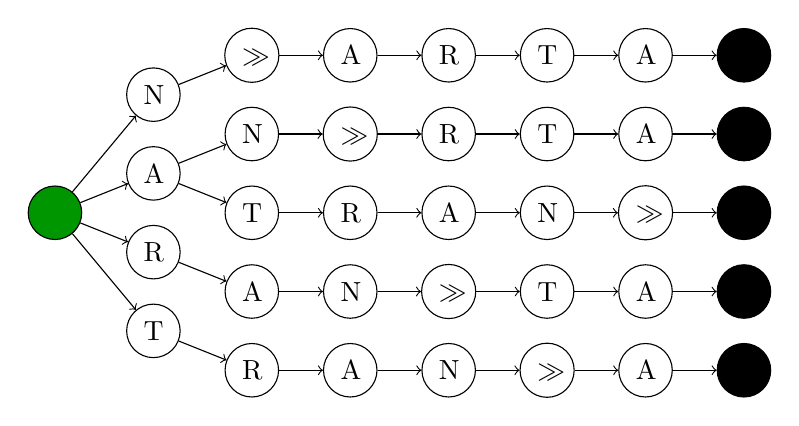
\begin{tikzpicture}
		\tikzstyle{every node}=[draw, shape=circle, minimum width = 15pt, minimum height = 15pt, text height = 7pt, text width = 7pt, align = center];
		\node [fill=UniGreen] (root) at (0,0) {};
		\node (n01) at (1.25, 1.5) {N};
		\node (n02) at (1.25, 0.5) {A};
		\node (n03) at (1.25, -0.5) {R};
		\node (n04) at (1.25, -1.5) {T};
		\node (n11) at (2.5, 2) {$\gg$};
		\node (n12) at (2.5, 1) {N};
		\node (n13) at (2.5, 0) {T};
		\node (n14) at (2.5, -1) {A};
		\node (n15) at (2.5, -2) {R};
		\node (n21) at (3.75, 2) {A};
		\node (n22) at (3.75, 1) {$\gg$};
		\node (n23) at (3.75, 0) {R};
		\node (n24) at (3.75, -1) {N};
		\node (n25) at (3.75, -2) {A};
		\node (n31) at (5, 2) {R};
		\node (n32) at (5, 1) {R};
		\node (n33) at (5, 0) {A};
		\node (n34) at (5, -1) {$\gg$};
		\node (n35) at (5, -2) {N};
		\node (n41) at (6.25, 2) {T};
		\node (n42) at (6.25, 1) {T};
		\node (n43) at (6.25, 0) {N};
		\node (n44) at (6.25, -1) {T};
		\node (n45) at (6.25, -2) {$\gg$};
		\node (n51) at (7.5, 2) {A};
		\node (n52) at (7.5, 1) {A};
		\node (n53) at (7.5, 0) {$\gg$};
		\node (n54) at (7.5, -1) {A};
		\node (n55) at (7.5, -2) {A};
		\node [fill=black] (n61) at (8.75, 2) {};
		\node [fill=black] (n62) at (8.75, 1) {};
		\node [fill=black] (n63) at (8.75, 0) {};
		\node [fill=black] (n64) at (8.75, -1) {};
		\node [fill=black] (n65) at (8.75, -2) {};
		\draw[->] (root) -- (n01);
		\draw[->] (root) -- (n02);
		\draw[->] (root) -- (n03);
		\draw[->] (root) -- (n04);
		\draw[->] (n01) -- (n11);
		\draw[->] (n02) -- (n12);
		\draw[->] (n02) -- (n13);
		\draw[->] (n03) -- (n14);
		\draw[->] (n04) -- (n15);
		\draw[->] (n11) -- (n21);
		\draw[->] (n12) -- (n22);
		\draw[->] (n13) -- (n23);
		\draw[->] (n14) -- (n24);
		\draw[->] (n15) -- (n25);
		\draw[->] (n21) -- (n31);
		\draw[->] (n22) -- (n32);
		\draw[->] (n23) -- (n33);
		\draw[->] (n24) -- (n34);
		\draw[->] (n25) -- (n35);
		\draw[->] (n31) -- (n41);
		\draw[->] (n32) -- (n42);
		\draw[->] (n33) -- (n43);
		\draw[->] (n34) -- (n44);
		\draw[->] (n35) -- (n45);
		\draw[->] (n41) -- (n51);
		\draw[->] (n42) -- (n52);
		\draw[->] (n43) -- (n53);
		\draw[->] (n44) -- (n54);
		\draw[->] (n45) -- (n55);
		\draw[->] (n51) -- (n61);
		\draw[->] (n52) -- (n62);
		\draw[->] (n53) -- (n63);
		\draw[->] (n54) -- (n64);
		\draw[->] (n55) -- (n65);
	\end{tikzpicture}
\end{frame}

\begin{frame}
	\frametitle{GADDAG - wady}
	
	\begin{itemize}
	 \item Duża złożoność pamięciowa.
	 \item Można próbować minimalizować graf po węzłach zawierających $\gg$.
	\end{itemize}
	
	\vspace{1em}
	
	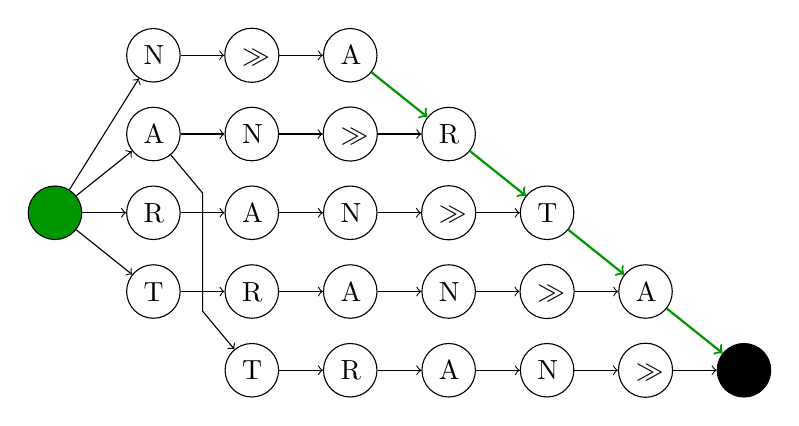
\begin{tikzpicture}
		\tikzstyle{every node}=[draw, shape=circle, minimum width = 15pt, minimum height = 15pt, text height = 7pt, text width = 7pt, align = center];
		\node [fill=UniGreen] (root) at (0,0) {};
		\node (n01) at (1.25, 2) {N};
		\node (n02) at (1.25, 1) {A};
		\node (n03) at (1.25, 0) {R};
		\node (n04) at (1.25, -1) {T};
		\node (n11) at (2.5, 2) {$\gg$};
		\node (n12) at (2.5, 1) {N};
		\node (n13) at (2.5, -2) {T};
		\node (n14) at (2.5, 0) {A};
		\node (n15) at (2.5, -1) {R};
		\node (n21) at (3.75, 2) {A};
		\node (n22) at (3.75, 1) {$\gg$};
		\node (n23) at (3.75, -2) {R};
		\node (n24) at (3.75, 0) {N};
		\node (n25) at (3.75, -1) {A};
		\node (n32) at (5, 1) {R};
		\node (n33) at (5, -2) {A};
		\node (n34) at (5, 0) {$\gg$};
		\node (n35) at (5, -1) {N};
		\node (n43) at (6.25, -2) {N};
		\node (n44) at (6.25, 0) {T};
		\node (n45) at (6.25, -1) {$\gg$};
		\node (n53) at (7.5, -2) {$\gg$};
		\node (n55) at (7.5, -1) {A};
		\node [fill=black] (n63) at (8.75, -2) {};
		\draw[->] (root) -- (n01);
		\draw[->] (root) -- (n02);
		\draw[->] (root) -- (n03);
		\draw[->] (root) -- (n04);
		\draw[->] (n01) -- (n11);
		\draw[->] (n02) -- (n12);
		\draw[->] (n02) -- (1.875, 0.25) -- (1.875, -1.25) -- (n13);
		\draw[->] (n03) -- (n14);
		\draw[->] (n04) -- (n15);
		\draw[->] (n11) -- (n21);
		\draw[->] (n12) -- (n22);
		\draw[->] (n13) -- (n23);
		\draw[->] (n14) -- (n24);
		\draw[->] (n15) -- (n25);
		\draw[->] (n22) -- (n32);
		\draw[->] (n23) -- (n33);
		\draw[->] (n24) -- (n34);
		\draw[->] (n25) -- (n35);
		\draw[->] (n33) -- (n43);
		\draw[->] (n34) -- (n44);
		\draw[->] (n35) -- (n45);
		\draw[->] (n43) -- (n53);
		\draw[->] (n45) -- (n55);
		\draw[->] (n53) -- (n63);
		\draw[->, color=UniGreen, thick] (n21) -- (n32);
		\draw[->, color=UniGreen, thick] (n32) -- (n44);
		\draw[->, color=UniGreen, thick] (n44) -- (n55);
		\draw[->, color=UniGreen, thick] (n55) -- (n63);
		\end{tikzpicture}
\end{frame}

\section{Przegląd aplikacji}

\begin{frame}
	\frametitle{Maven i~Quackle - porównanie}
	
		\scalebox{0.7}{
		\begin{tabular}{|l|c|c|}
			\cline{2-3}
			\multicolumn{1}{c|}{} & \textbf{Maven} & \textbf{Quackle} \\
			\hline
			\multirow{2}{*}{Autorzy} & \multirow{2}{*}{Brian Sheppard} & Jason Katz-Brown,  \\
			&& John O'Laughlin \\
			\hline
			Źródło & Zamknięte & Otwarte (C++, Qt) \\
			\hline
			Struktura słownika & DAWG & GADDAG \\
			\hline
			\multirow{3}{*}{Strategia} & Zależna od fazy gry. Wykorzystanie &  Zależna od fazy gry. Wykorzystanie \\
			& heurystyk i~symulacji do ewaluacji & heurystyk i~symulacji do ewaluacji \\
			& najbardziej korzystnych ruchów. & najbardziej korzystnych ruchów. \\
			\hline
			Wyniki przeciwko & \multicolumn{1}{l|}{\textcolor{UniGreen}{$\blacktriangleright$} 9-5 vs Adam Logan (1997)} & \multicolumn{1}{l|}{\textcolor{UniGreen}{$\blacktriangleright$} 3-2 vs David Boys (2006)} \\
			ludziom & \multicolumn{1}{l|}{\textcolor{UniGreen}{$\blacktriangleright$} 6-3 vs Joel Sherman (2006)} &  \\
			\hline
			,,Bezpośrednie'' starcie & \multicolumn{1}{l|}{\textcolor{UniGreen}{$\blacktriangleright$} 30-6} & \multicolumn{1}{l|}{\textcolor{UniGreen}{$\blacktriangleright$} 32-4}  \\
			\hline
		\end{tabular}
	}
	
	\vspace{3em}
	
	\begin{center}
		,,It's still better to be a human than to be a computer'' - David Boys
	\end{center}
\end{frame}

\subsection{Strategia}

\begin{frame}
	\frametitle{Fazy gry}
	
	\begin{enumerate}
		\item \textbf{MG} - mid-game:
			\begin{itemize}
				\item Trwa od momentu rozpoczęcia gry, aż do osiągnięcia fazy pre-endgame.
			\end{itemize}
		\item \textbf{PEG} - pre-endgame.
			\begin{itemize}
				\item Dzieli się na dwa etapy - PEG-1 oraz PEG-2.
				\item Występuje, gdy do pobrania pozostają odpowiednio jedna lub dwie płytki.
				\item Przez PEG przechodzi ponad połowa gier.
			\end{itemize}
		\item \textbf{EG} - endgame.
			\begin{itemize}
				\item Rozpoczyna się, gdy pobrane zostaną wszystkie płytki.
				\item Wiadomo jakimi literami dysponuje przeciwnik.
			\end{itemize}
	\end{enumerate}
\end{frame}

\begin{frame}
	\frametitle{Mid-game (Quackle)}
	

\end{frame}

\subsection{Przeszukiwanie przestrzeni stanów}

\begin{frame}
	\frametitle{(Pre-)Endgame}

	\begin{columns}
		\begin{column}{.5\textwidth}
			\begin{itemize}
				\item W~fazach PEG, EG możliwe jest zastosowanie wyszukiwania wyczerpującego przestrzeni stanów.
				\item Algorytmy przeszukiwania $\alpha - \beta$, $A^{*}$, $B^{*}$.
				\item Obliczenia progresywne - przeszukiwanie rozpoczynane w~miejscu, w~którym można podjąć szybką i~pewną decyzję.
			\end{itemize}
		\end{column}
		\begin{column}{.5\textwidth}
			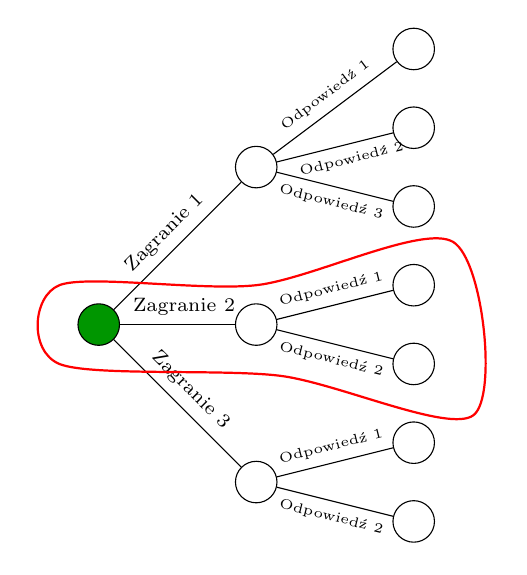
\begin{tikzpicture}
				\tikzstyle{state} = [draw, shape=circle, minimum width=15pt, minimum height=15pt]
				\node (s0) [state, fill=UniGreen] at (0,0) {};
				\node (s1) [state] at (2,2) {};
				\node (s2) [state] at (2,0) {};
				\node (s3) [state] at (2, -2) {};
				\node (s4) [state] at (4,3.5) {};
				\node (s5) [state] at (4,2.5) {};
				\node (s6) [state] at (4,1.5) {};
				\node (s7) [state] at (4,0.5) {};
				\node (s8) [state] at (4,-0.5) {};
				\node (s9) [state] at (4,-1.5) {};
				\node (s10) [state] at (4,-2.5) {};
				\draw (s0) -- node[above, sloped, font=\scriptsize] {Zagranie 1} (s1);
				\draw (s0) -- node[above, sloped, font=\scriptsize, near end, xshift=-8pt] {Zagranie 2} (s2);
				\draw (s0) -- node[above, sloped, font=\scriptsize] {Zagranie 3} (s3);
				\draw (s1) -- node[above, sloped, font=\tiny] {Odpowiedź 1} (s4);
				\draw (s1) -- node[xshift=-6pt, below, near end, sloped, font=\tiny] {Odpowiedź 2} (s5);
				\draw (s1) -- node[below, sloped, font=\tiny] {Odpowiedź 3} (s6);
				\draw (s2) -- node[above, sloped, font=\tiny] {Odpowiedź 1} (s7);
				\draw (s2) -- node[below, sloped, font=\tiny] {Odpowiedź 2} (s8);
				\draw (s3) -- node[above, sloped, font=\tiny] {Odpowiedź 1} (s9);
				\draw (s3) -- node[below, sloped, font=\tiny] {Odpowiedź 2} (s10);
				\draw [red, thick] plot [smooth cycle] coordinates {(-0.5, -0.5) (-0.5, 0.5) (2, 0.5) (4.5, 1.05) (4.76, -1.15) (2.3, -0.65)};
			\end{tikzpicture}
		\end{column}
	\end{columns}
\end{frame}

\section{Podsumowanie}
\subsection{Literatura}

\begin{frame}
	\frametitle<presentation>{Literatura}
	\begin{thebibliography}{10}
		\beamertemplatearticlebibitems
			\bibitem{ScrabblePSPACE}
    		M.~Lampis, V.~Mitsou, K.~Sołtys.
    		\newblock Scrabble is PSPACE-Complete.

		\beamertemplatebookbibitems
			\bibitem{WCCS}
			Brian Sheppard.
			\newblock World-championship-caliber Scrabble.
			\newblock {\em Artificial Intelligence}, vol. 134, p. 241-275, January 2002.
  		
  		\beamertemplatearticlebibitems
  			\bibitem{Quackle2005}
  			J.~Katz-Brown, J.~O'Laughlin.
    		\newblock How Quackle Plays Scrabble.
	\end{thebibliography}
\end{frame}

\subsection{Zakończenie}

\begin{frame}
	\begin{center}
		\LARGE{\textbf{Dziękuję za uwagę!}}
	\end{center}
\end{frame}

\end{document}